\documentclass{beamer}
\usetheme{CambridgeUS}
% Đặt màu cho các block
\setbeamercolor{block title}{bg=red!80!black, fg=white}
\setbeamercolor{block body}{bg=red!10, fg=black}
%%%%%%%%%%%%%%%%%%%%%%%%%%%%%%%%%%%%%%%%%%%%%%%%%%%%%%%
\usepackage[utf8]{vietnam}
% Dùng để thêm hình ảnh
\usepackage{graphicx}
% Dùng để di chuyển các tham chiếu
\usepackage{hyperref}
% Dùng để tạo văn bản ngẫu nhiên
\usepackage{lipsum}
% \usepackage{xcolor}
%%%%%%%%%%%%%%%%%%%%%%%%%%%%%%%%%%%%%%%%%%%%%%%%%%%%%%%
\AtBeginSection[]
{
\begin{frame}<beamer>
\frametitle{Nội dung}

\tableofcontents[
currentsection,
subsectionstyle=hide/hide,
subsubsectionstyle=hide/hide
]

\end{frame}
}

% \AtBeginSubsection[]
% {
% \begin{frame}<beamer>
% \frametitle{Nội dung}

% \tableofcontents[
% currentsection,
% currentsubsection,
% subsectionstyle=show/shaded/hide,
% subsubsectionstyle=show/show/shaded/hide
%]

% \end{frame}
%}
%%%%%%%%%%%%%%%%%%%%%%%%%%%%%%%%%%%%%%%%%%%%%%%%%%%%%%%
\title[{\makebox[.15\paperwidth]{Human Resources Management}}]{Chủ đề: Human Resources Management}
\author[Nhóm 22]{Nhóm 22}
\date[Data Warehouse \& BI]{\today}
%%%%%%%%%%%%%%%%%%%%%%%%%%%%%%%%%%%%%%%%%%%%%%%%%%%%%%%
\begin{document}
%%%%%%%%%%%%%%%%%%%%%%%%%%%%%%%%%%%%%%%%%%%%%%%%%%%%%%%
\begin{frame}
\titlepage
\end{frame}
%%%%%%%%%%%%%%%%%%%%%%%%%%%%%%%%%%%%%%%%%%%%%%%%%%%%%%%
\begin{frame}{Thành viên nhóm}
\begin{block}{Nhóm 22}
\centering
\begin{tabular} {|l|c|}
\hline
Họ và tên & MSSV \\
\hline
Nguyễn Việt Anh & 20216796 \\
Phùng Quốc Đạt & 20216813 \\
Vũ Văn Nghĩa & 20206205 \\
Mai Thị Tuyết Nhung & 20216866 \\
\hline
\end{tabular}
\end{block}
\end{frame}
%%%%%%%%%%%%%%%%%%%%%%%%%%%%%%%%%%%%%%%%%%%%%%%%%%%%%%%
%%%%%%%%%%%%%%%%%%%%%%%%%%%%%%%%%%%%%%%%%%%%%%%%%%%%%%%
%%%%%%%%%%%%%%%%%%%%%%%%%%%%%%%%%%%%%%%%%%%%%%%%%%%%%%%
%%%%%%%%%%%%%%%%%%%%%%%%%%%%%%%%%%%%%%%%%%%%%%%%%%%%%%%
%%%%%%%%%%%%%%%%%%%%%%%%%%%%%%%%%%%%%%%%%%%%%%%%%%%%%%%
\section{Khảo sát}
\subsection{Giới thiệu về HRM}

\begin{frame}{Giới thiệu về HRM}
\begin{columns}

\begin{column}{0.4\textwidth}

\includegraphics[width=\textwidth]{pictures/Giới thiệu về HRM.jpg}
\end{column}

\begin{column}{0.6\textwidth}
\begin{itemize}
\item HRM là gì?
\item HRM là gì?
\item \dots
% https://talentbold.com/hrm-la-gi-tat-tan-tat-ve-human-resource-management-939-ns
% https://en.wikipedia.org/wiki/Human_resource_management
\end{itemize}
\end{column}

\end{columns}
\end{frame}
%%%%%%%%%%%%%%%%%%%%%%%%%%%%%%%%%%%%%%%%%%%%%%%%%%%%%%%
\subsection{Business Model Canvas}
\begin{frame}{Business Model Canvas}
\begin{figure}[H]
\centering
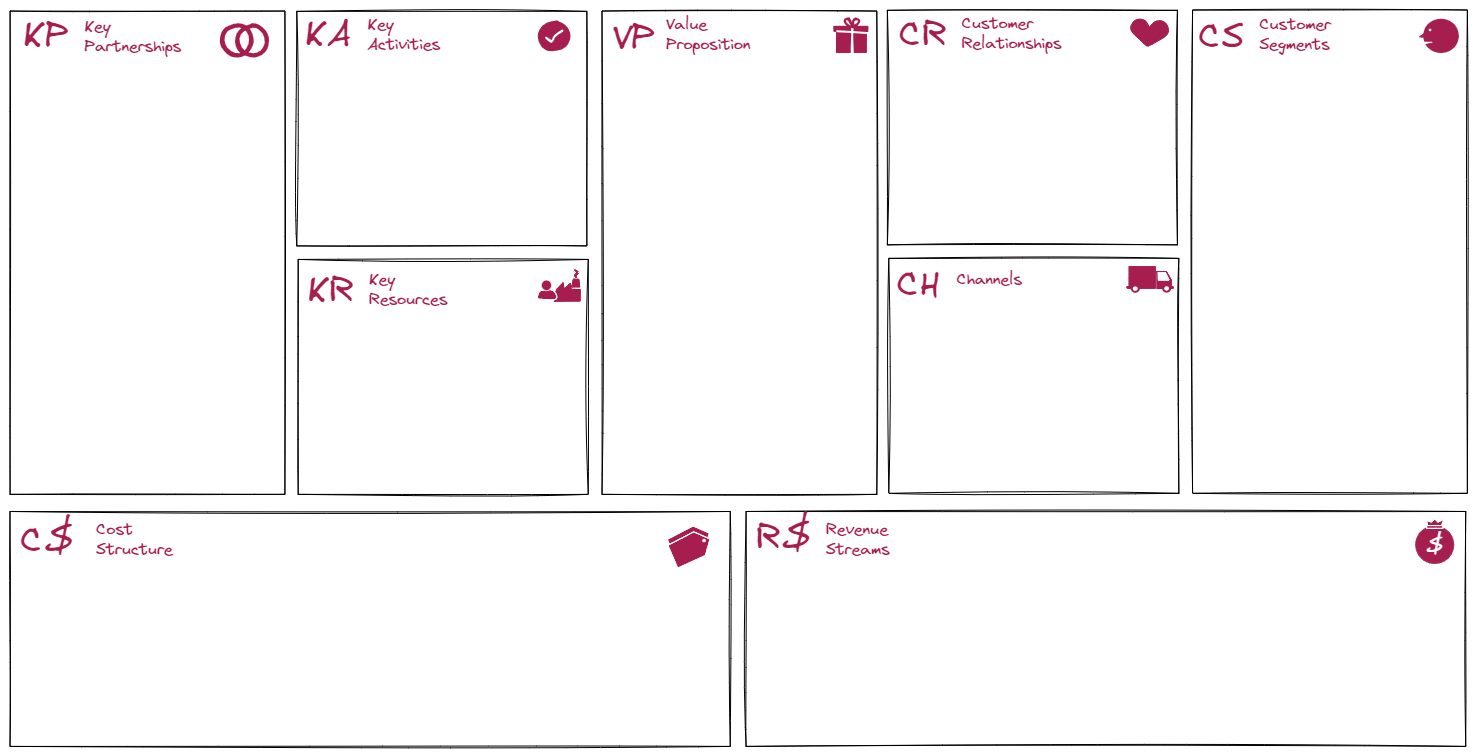
\includegraphics[scale = 0.2]{pictures/Business Model Canvas.excalidraw.png}
\end{figure}
\end{frame}
%%%%%%%%%%%%%%%%%%%%%%%%%%%%%%%%%%%%%%%%%%%%%%%%%%%%%%%
\section{Phân tích và Thiết kế}

% ETL bbb aaaa BEFORE AFTER

% achitect DATA ARCHITECTURE
% \caption{Thực hành xây dựng kiến trúc hệ thống phân tích dữ liệu}


\begin{frame}{xxxxxxxxxxxxx}
\begin{itemize}
\item Nội dung xxxxxxxxxxxxx
\end{itemize}
\end{frame}
%%%%%%%%%%%%%%%%%%%%%%%%%%%%%%%%%%%%%%%%%%%%%%%%%%%%%%%
\section{Xây dựng Dashboard}
\begin{frame}{xxxxxxxxxxxxx}
\begin{itemize}
\item Nội dung xxxxxxxxxxxxx
\end{itemize}
\end{frame}
%%%%%%%%%%%%%%%%%%%%%%%%%%%%%%%%%%%%%%%%%%%%%%%%%%%%%%%
\section{Tổng kết}
\begin{frame}{xxxxxxxxxxxxx}
\begin{itemize}
\item Nội dung xxxxxxxxxxxxx
\end{itemize}
\end{frame}
%%%%%%%%%%%%%%%%%%%%%%%%%%%%%%%%%%%%%%%%%%%%%%%%%%%%%%%

%%%%%%%%%%%%%%%%%%%%%%%%%%%%%%%%%%%%%%%%%%%%%%%%%%%%%%%
%%%%%%%%%%%%%%%%%%%%%%%%%%%%%%%%%%%%%%%%%%%%%%%%%%%%%%%
%%%%%%%%%%%%%%%%%%%%%%%%%%%%%%%%%%%%%%%%%%%%%%%%%%%%%%%
%%%%%%%%%%%%%%%%%%%%%%%%%%%%%%%%%%%%%%%%%%%%%%%%%%%%%%%
%%%%%%%%%%%%%%%%%%%%%%%%%%%%%%%%%%%%%%%%%%%%%%%%%%%%%%%
\section*{}
\begin{frame}{}
\centering
\Huge{Thanks for listening!}
\end{frame}
%%%%%%%%%%%%%%%%%%%%%%%%%%%%%%%%%%%%%%%%%%%%%%%%%%%%%%%
\end{document}
%%%%%%%%%%%%%%%%%%%%%%%%%%%%%%%%%%%%%%%%%%%%%%%%%%%%%%%
\begin{frame}{xxxxxxxxxxxxx}

\begin{columns}
\begin{column}{0.49\textwidth}

\begin{itemize}
\item xxxxxxxxxxxxx
\item xxxxxxxxxxxxx
\item xxxxxxxxxxxxx
\end{itemize}
\end{column}

\begin{column}{.02\textwidth}
\rule{.1mm}{0.7\textheight}
\end{column}

\begin{column}{0.49\textwidth}

\begin{itemize}
\item xxxxxxxxxxxxx
\item xxxxxxxxxxxxx
\item xxxxxxxxxxxxx
\end{itemize}
\end{column}

\end{columns}
\end{frame}
%%%%%%%%%%%%%%%%%%%%%%%%%%%%%%%%%%%%%%%%%%%%%%%%%%%%%%%

https://www.kaggle.com/code/colara/human-resources-analytics-a-descriptive-analysis
https://www.kaggle.com/datasets/rishikeshkonapure/hr-analytics-prediction
https://www.kaggle.com/code/jacksonchou/hr-analytics
https://www.kaggle.com/datasets/davidepolizzi/hr-data-set-based-on-human-resources-data-set
https://www.kaggle.com/datasets/rhuebner/human-resources-data-set
https://www.kaggle.com/code/sayamkumar/employee-attrition-prediction/input

https://www.kaggle.com/docs/api
https://www.kaggle.com/datasets/rhuebner/human-resources-data-set/data
https://www.kaggle.com/datasets/sherrytp/airline-delay-analysis?fbclid=IwAR2wsZkBGKgSIZj29PQLxTqLvoqG9HuLFjCWxrKztTzGRuGAOG5EiqqhvVg

https://downloadlynet.ir/2024/28/116039/01/machine-learning-data-science-with-python-kaggle-pandas/20/?#/116039-udemy-182411021524.html
https://downloadlynet.ir/2024/28/116043/01/machine-learning-data-science-with-python-kaggle-a-z/21/?#/116043-udemy-182411020524.html
%%%%%%%%%%%%%%%%%%%%%%%%%%%%%%%%%%%%%%%%%%%%%%%%%%%%%%%